\subsection{The diffractometer}

\begin{figure}
	\centering
	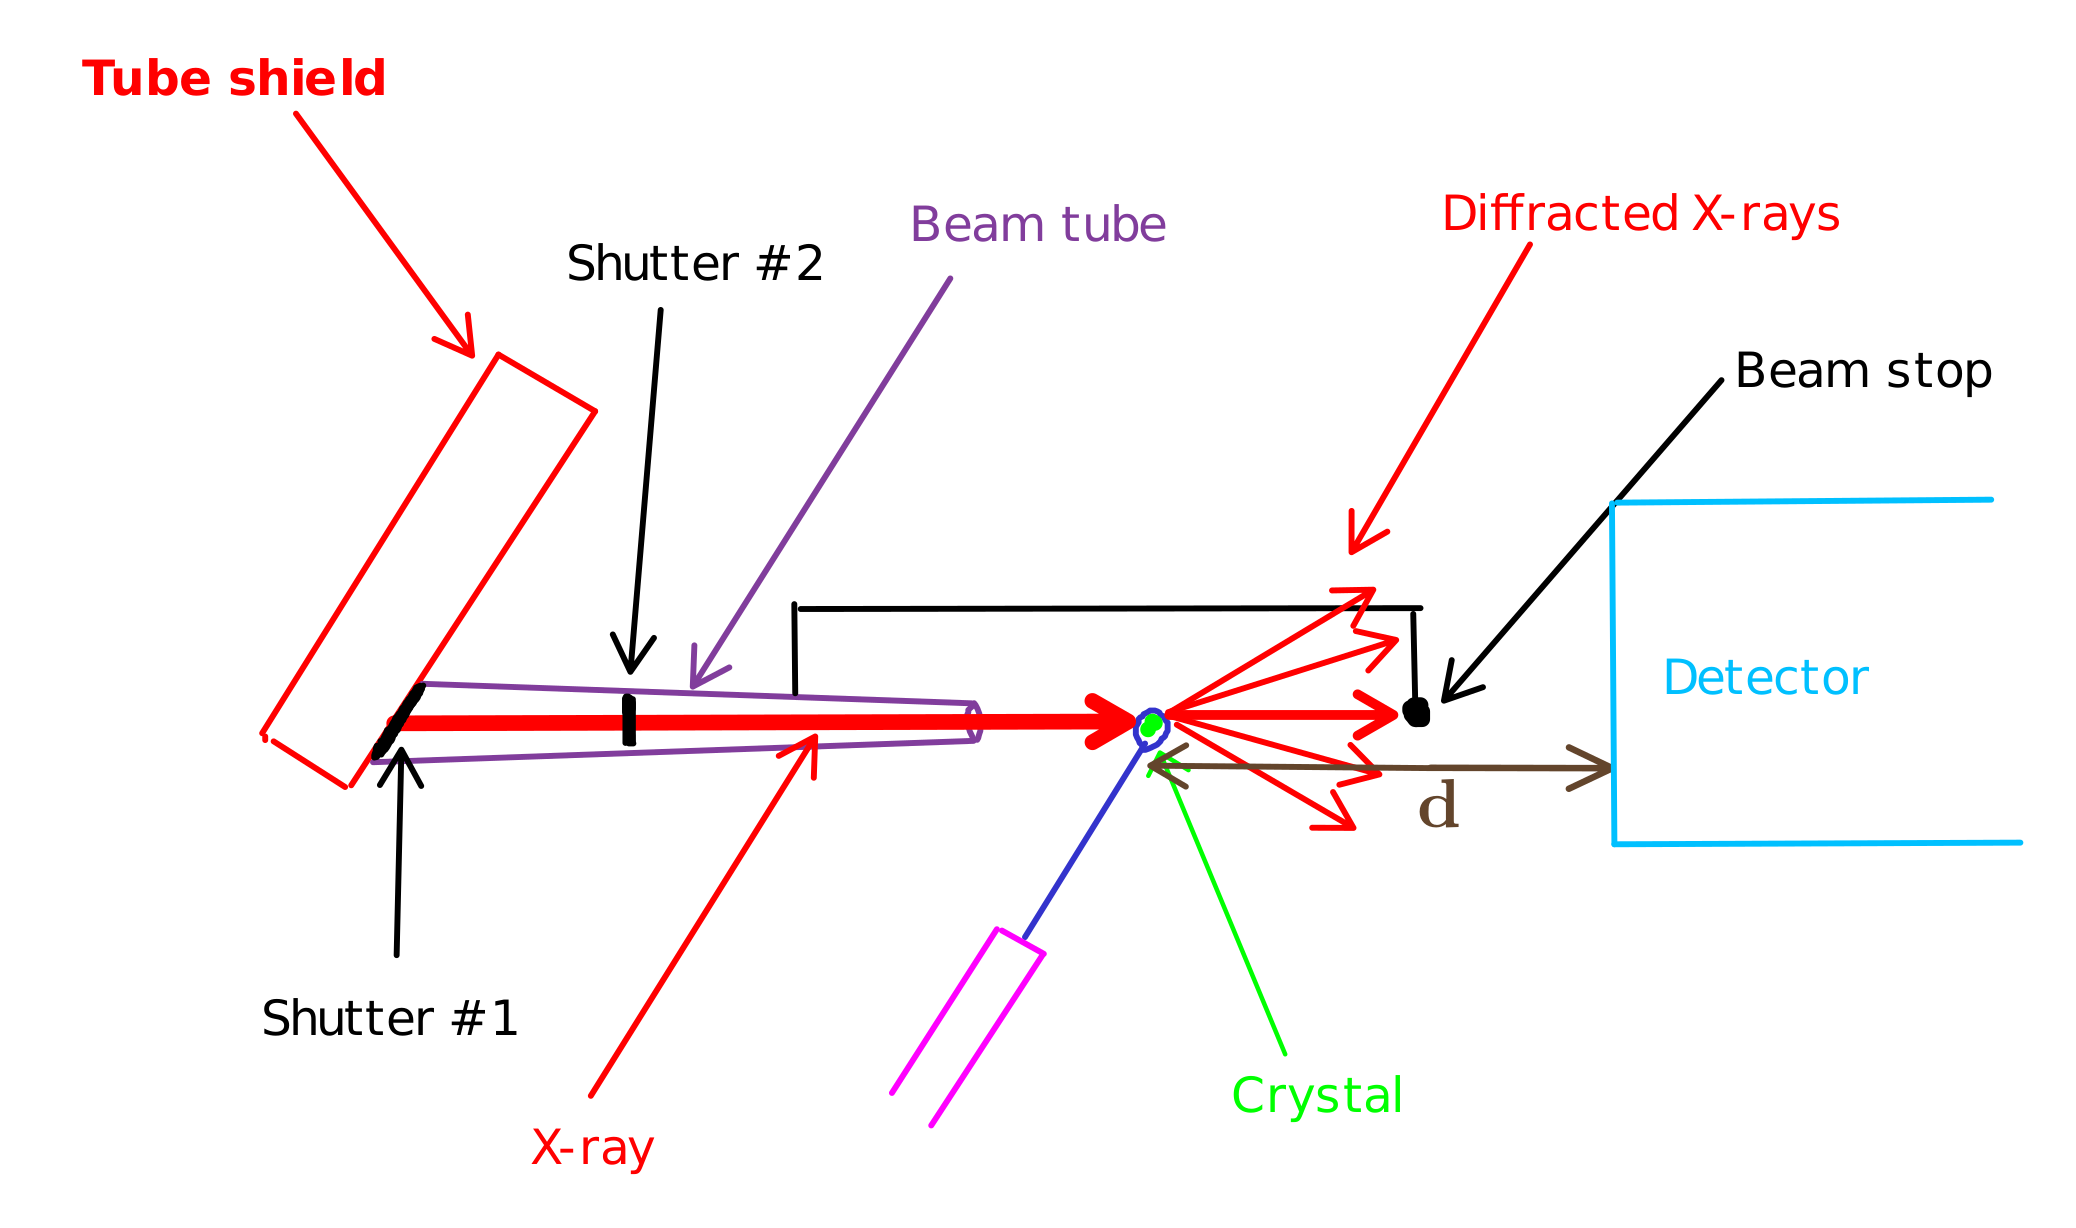
\includegraphics[scale=0.15]{sc_diffractometer_lateral.png}
	\caption{\label{diffractometer_lateral}Lateral view of a SCXRD diffractometer. See text for details.}
\end{figure}

Figure~\ref{diffractometer_lateral} is a lateral schematic of the diffractometer. The X-rays are generated within the tube shield and are emitted through the transparent Be window. When we physically work with the diffractometer, for example, to mount the crystal, we do not want the X-rays in the diffractometer chamber. Shutter \# 1 on the tube shield is used to stop the X-rays from coming out of the tube shield. The beam pipe contains the beam optics, which consists of the $K_\beta$ filter, collimation optics, as well as another shutter. This shutter controls the exposure time.

The intensity of the generated X-rays is very high, and all of the intensity is not diffracted by the crystal. A portion of the X-ray beam transmits through the crystal and directly hits the detector if it is at $2\theta = 0.$ This high intensity beam can damage the detector. The beam stop prevents the direct beam from falling on the detector. For a typical beam of spot size $\SI{0.5}{mm}$ diameter, the beam stop is $\sim \SI{2}{mm}.$ In Fig.~\ref{fig:rotation_photo}, the dark portion is the shadow of this beam stop.

The distance between the detector and the crystal, denoted by $d,$ is generally kept $4-10~\si{cm},$ and the detector can move back upto $\SI{18}{cm}.$ The intensity of the diffracted beam falls off $\propto \dfrac{1}{d^6}.$ Hence, if $d$ is large, exposure time will increase. $d$ depends on the lattice parameters of the crystal:%
%	
	\begin{subequations}
		\begin{align}
		d \sim \begin{cases}
		\SI{4}{cm} & \text{for } a, b, c < 12-13~\si{\angstrom};\\
		5-6~\si{cm} & \text{for } a, b, c < 12-30~\si{\angstrom};\\
		7-8~\si{cm} & \text{for } a, b, c > \SI{30}{\angstrom}.\\
		\end{cases}
		\end{align}
	\end{subequations}
	
\begin{figure}
	\centering
	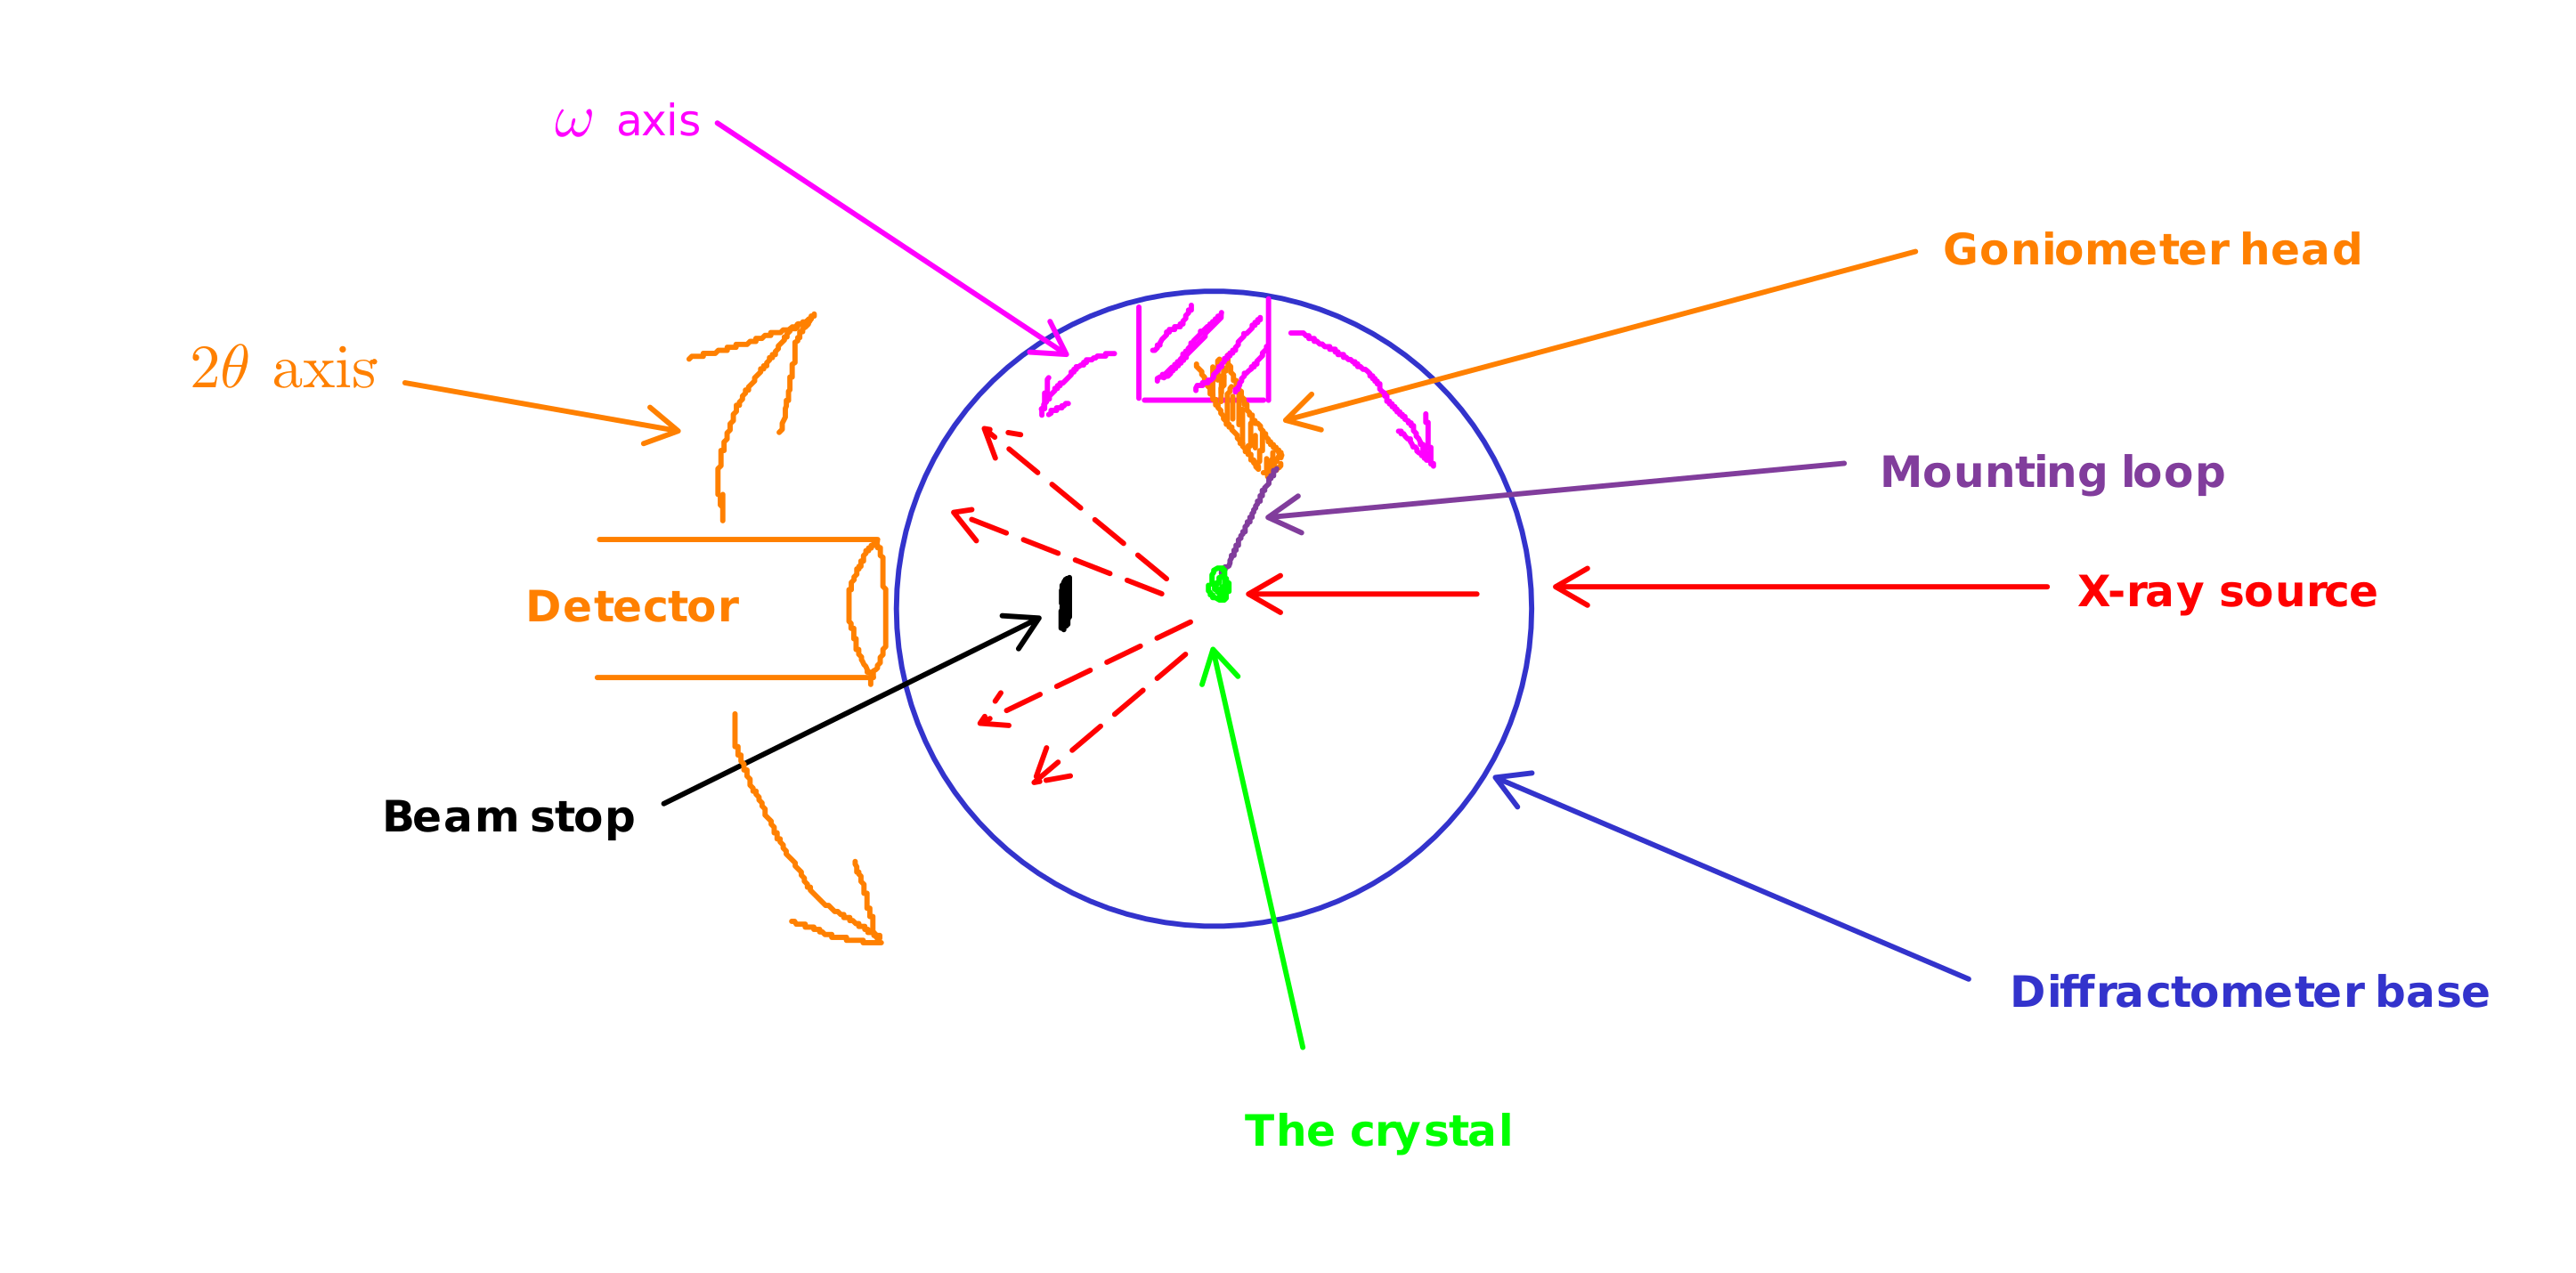
\includegraphics[scale=0.2]{sc_diffractometer_omega.png}
	\caption{\label{diffractometer_omega}Top view of a SCXRD diffractometer. The $\omega$ axis is the rotation axis of the diffractometer base. $2\theta$ is the angle of rotation of the detector.}
\end{figure}
	
\begin{figure}
	\centering
	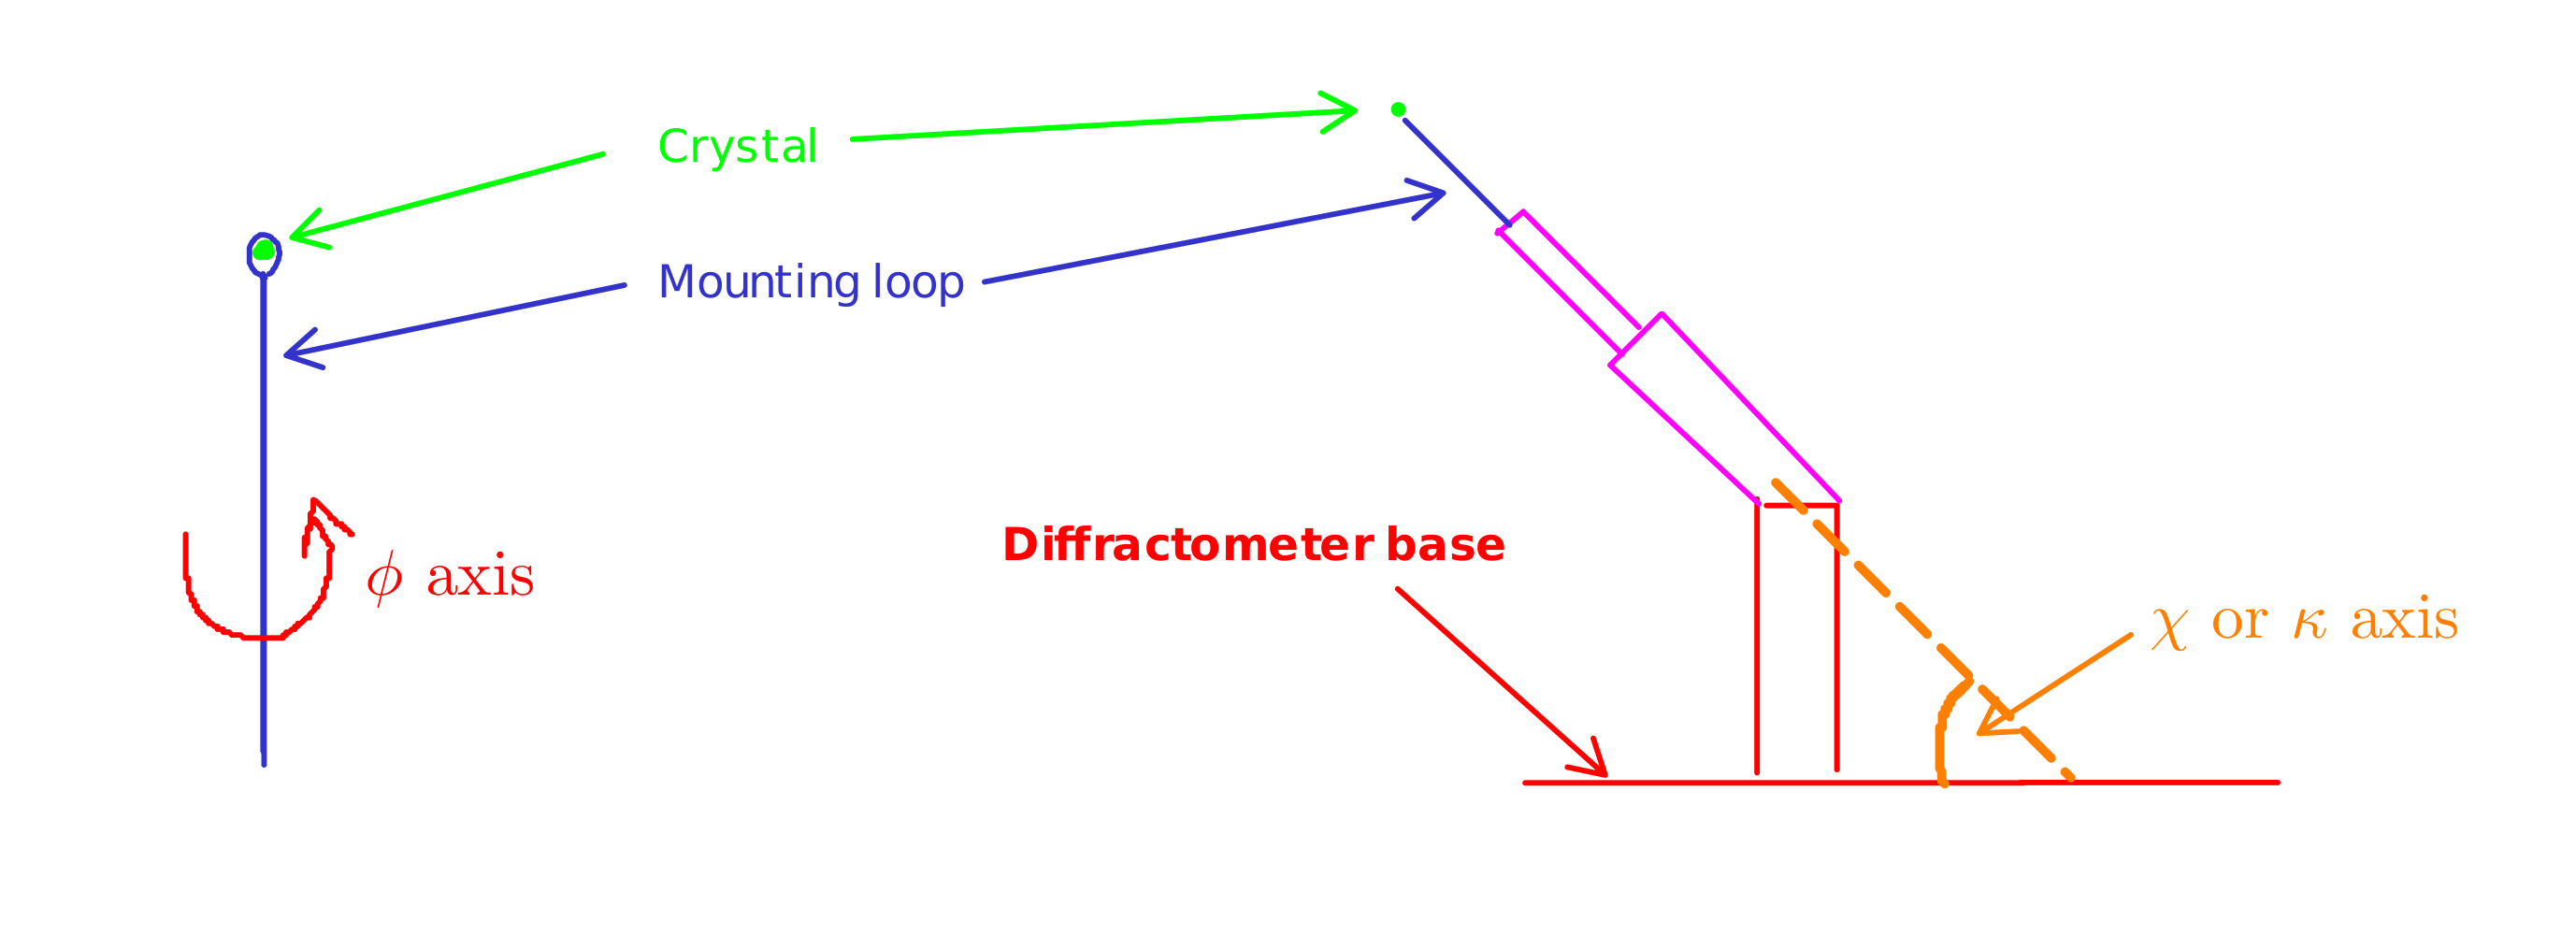
\includegraphics[width=\textwidth]{sc_diffractometer_phi_chi.png}
	\caption{\label{diffractometer_phi_chi}The $\phi$ axis is the rotation axis of the crystal about the mounting loop. If the angle that the goniometer makes with the diffractometer base is fixed, then the angle is termed as the $\chi$ axis, with $\chi = \SI{54.7}{\degree}.$ If this angle can be changed, then the same axis is known as the $\kappa$ axis.}
\end{figure}

\begin{figure}
	\centering
	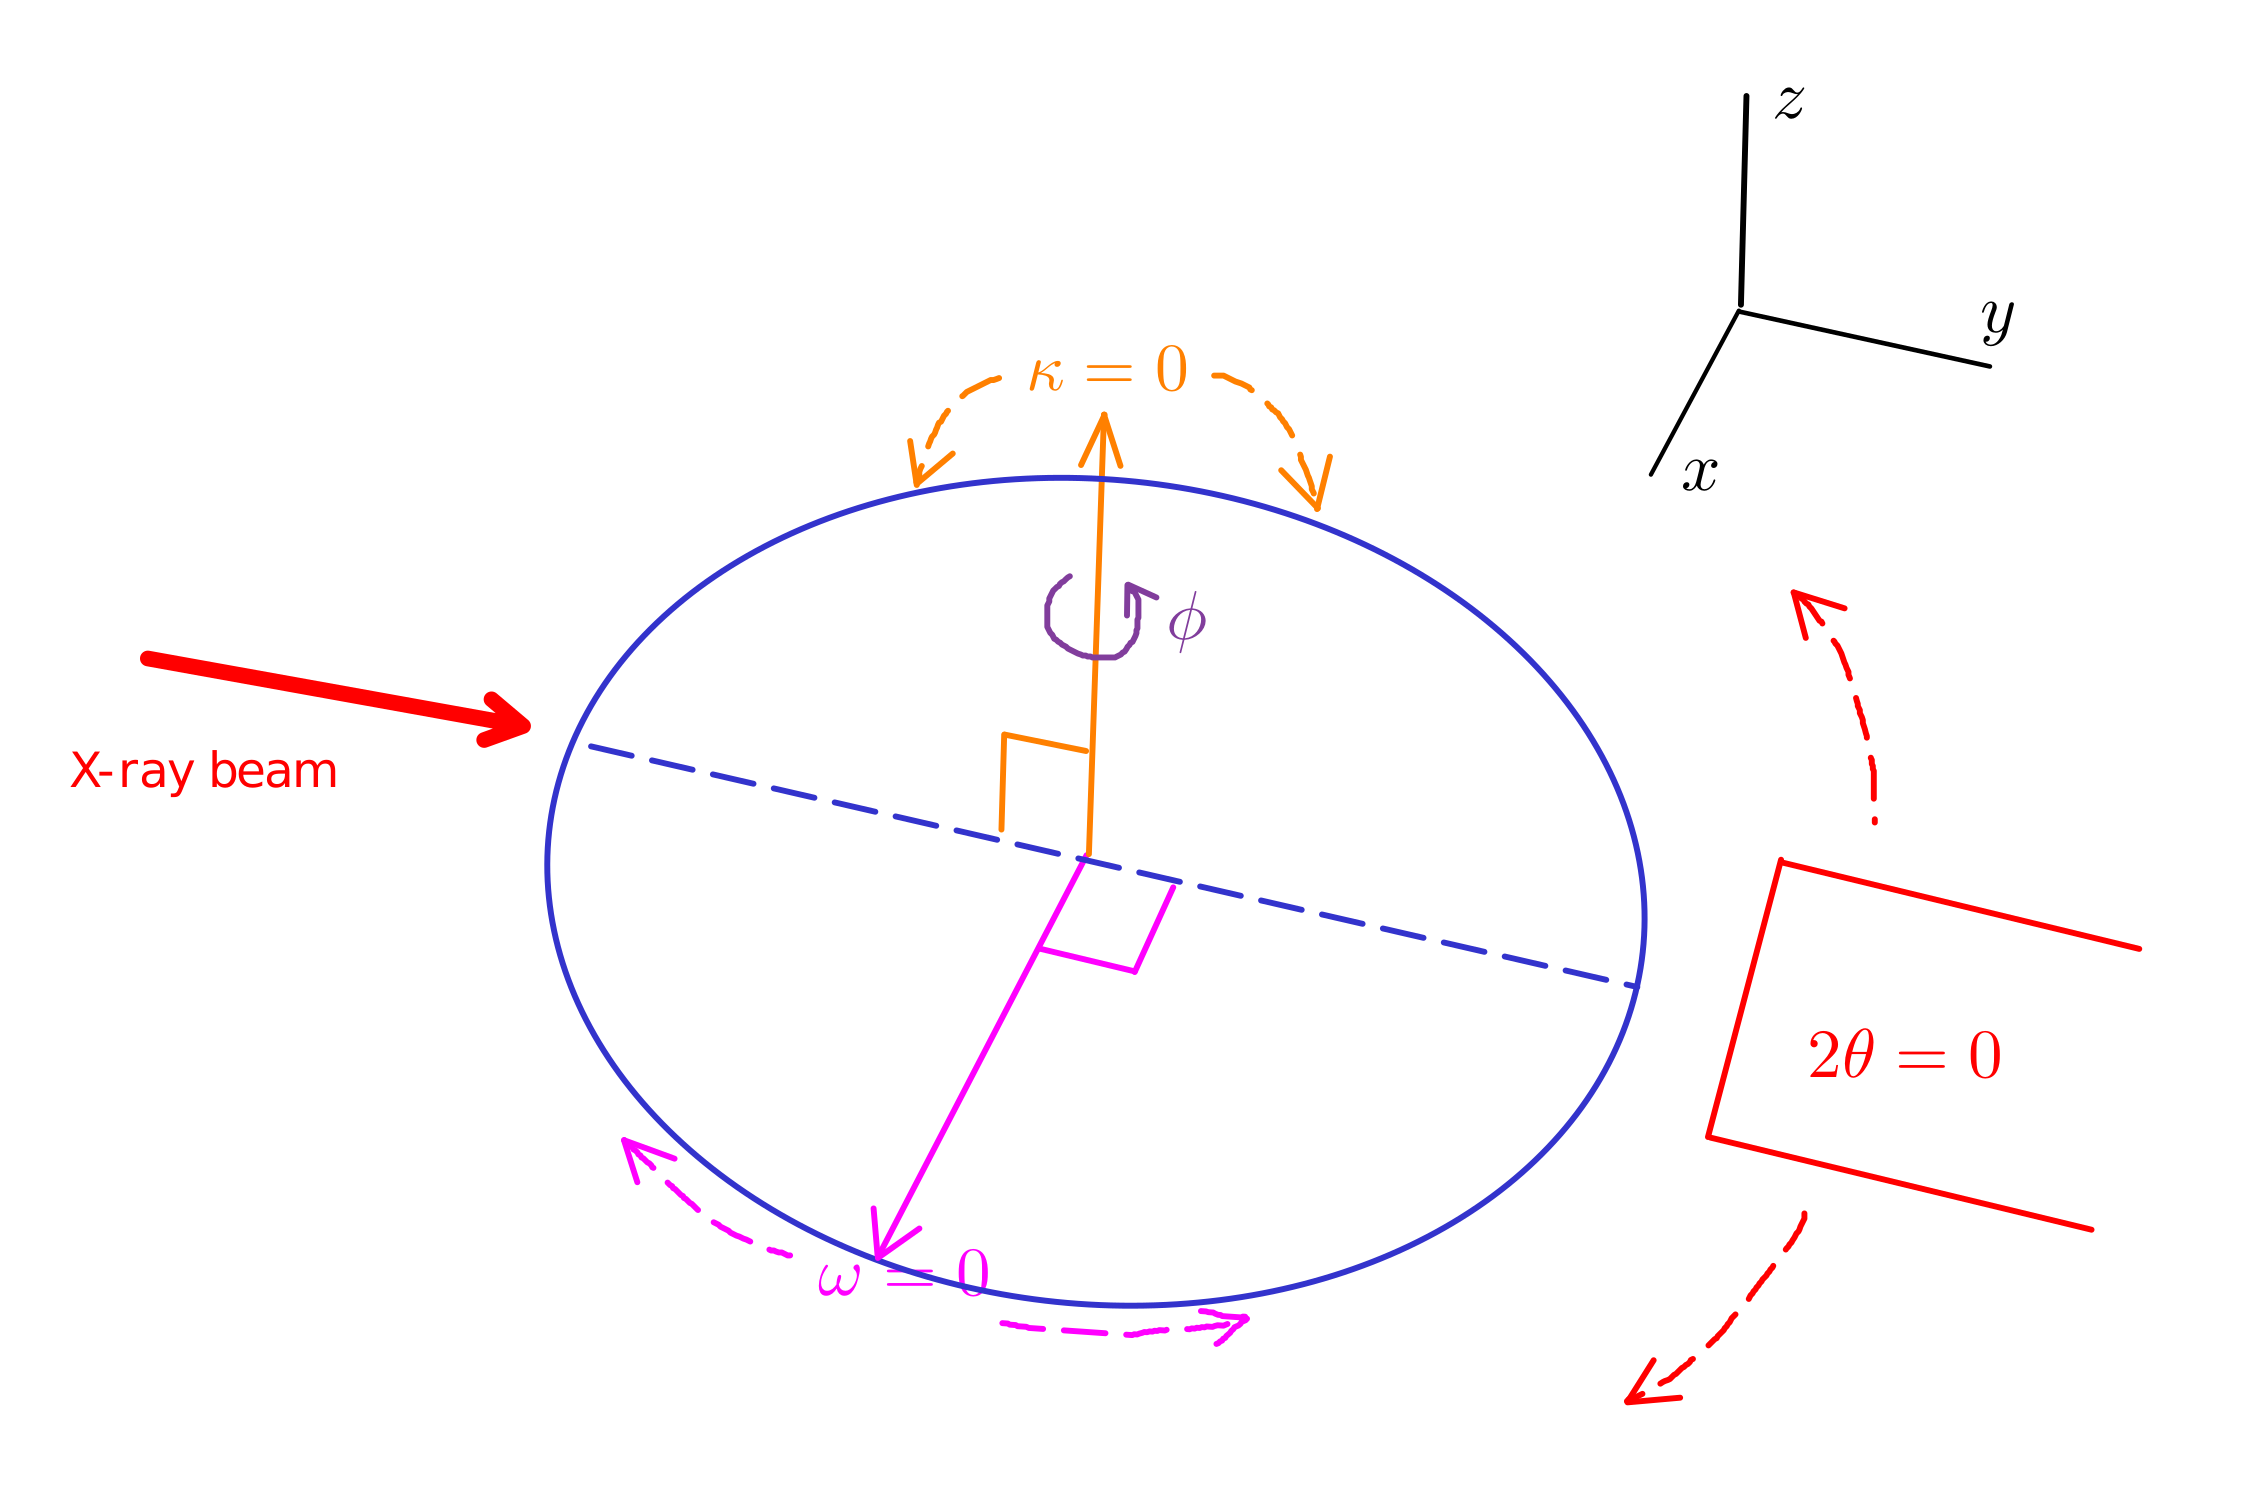
\includegraphics[scale=0.15]{all_axes.png}
	\caption{\label{diffractometer_all_axes}All the axes of a single crystal diffractometer.}
\end{figure}
 
A diffractometer can have four axes of rotation:%
%	
	\begin{enumerate}%
%	
	    \item $\phi$ axis,
	    
	    \item $\omega$ axis,
	    
	    \item $\chi$ or $\kappa$ axis, and
	    
	    \item $2\theta$ axis.
	    
	\end{enumerate}

These axis are shown in figures~\ref{diffractometer_omega}, \ref{diffractometer_phi_chi} and \ref{diffractometer_all_axes}.\\

Based on this, SCXRD diffractometers can be classified into:%
%	
	\begin{itemize}%
%	
	    \item \ul{2-circle diffractometer}: $\phi$ and $\omega$ can be varied, but $\chi$ and $2\theta$ are fixed. $2\theta$ is fixed at $\SI{30}{\degree}.$ But the coverage area of the detector is such that if it sits at $\SI{30}{\degree},$ it can actually reach $0-60\si{\degree}.$ For $\mathrm{Mo}~K_\alpha$ radiation, the IUCr prescribed minimum $2\theta = \SI{50}{\degree}.$ So, a 2-circle diffractometer works fine for $\mathrm{Mo}~K_\alpha$ radiation. We can, however, not go to higher angles, so this diffractometer is used for routine analysis of crystals.
	    
	    \item \ul{3-circle diffractometer}: $\phi$, $\omega$ and $2\theta$ can be varied. Allows data recording upto high angles.
	    
	    \item \ul{4-circle diffractometer}: $\phi$, $\omega$, $2\theta$ and $\kappa$ can be changed. Reduces data collection time because a large number of reflections can be brought to the periphery of the Ewald sphere.
	    
	\end{itemize}
	
\begin{table}
	\newcounter{sl_no}
	\centering
	\caption{\label{tab:3_circ_diff_angles}Standard measurement angles and exposure time for a 3-circle diffractometer. $\Delta \omega$ is the step size or width in $\omega.$ The full set represents a complete sphere of data; the first two sets are recorded with 200 frames of the third set correspond to a hemisphere of data.}
	\begin{tabular}{|c|C|C|C|C|C|C|C|}
		
		\hline
		
		Sl. No. & 2\theta & \omega & \phi & \multicolumn{1}{c|}{\makecell{$\chi$\\(Fixed)}} & \Delta \omega & \multicolumn{1}{c|}{\makecell{\text{No. of frames}}} & \multicolumn{1}{c|}{\makecell{\text{Exposure time}\\$t$ (in s)}}\\
		
		\hhline{|=|=|=|=|=|=|=|=|}
		
		\stepcounter{sl_no}\arabic{sl_no} & \SI{-30}{\degree} & \SI{-30}{\degree} & 0 & \SI{54.74}{\degree} & \SI{1}{\degree}/\SI{0.5}{\degree}/\SI{0.3}{\degree} & 180/360/600 & 5/10/15\\
		
		\hline
		
		\stepcounter{sl_no}\arabic{sl_no} & \SI{-30}{\degree} & \SI{-30}{\degree} & \SI{90}{\degree} & \SI{54.74}{\degree} & \SI{0.3}{\degree} & 600 & 10\\
		
		\hline
		
		\stepcounter{sl_no}\arabic{sl_no} & \SI{-30}{\degree} & \SI{-30}{\degree} & \SI{180}{\degree} & \SI{54.74}{\degree} & \SI{0.3}{\degree} & 600 & 10\\
		
		\hline
		
		\stepcounter{sl_no}\arabic{sl_no} & \SI{-30}{\degree} & \SI{-30}{\degree} & \SI{270}{\degree} & \SI{54.74}{\degree} & \SI{0.3}{\degree} & 600 & 10\\
		
		\hline
	
	\end{tabular}
\end{table}

	
Data collection strategies vary based on the type of diffractometer and the crystal being studied. Table~\ref{tab:3_circ_diff_angles} lists the standard angles which allow a full sphere of data to be collected using a 3-circle diffractometer. The exposure time is the time period for which the X-ray is allowed to fall on the crystal before its orientation is changed. The crystal is not kept stationary, instead, it is slowly rotated about the $\omega$ axis in steps of $\Delta\omega.$ A large value of $\Delta\omega$ implies that we are slicing the reciprocal lattice into wider slices. If we take $\Delta\omega = \SI{1}{\degree},$ it is recommended that we use a larger exposure time, so that the exposure time per degree remains fixed. Smaller values improve the quality of data. If $\chi$ (i.e. $\kappa$) can be varied, we can get the data faster.

Diffractometers have pre-fixed strategies that are used when an unknown crystal is loaded for the first time. This strategy cannot be edited, but may be extended in some cases. Using this strategy, 20-30 frames are recorded, from which the diffractometer informs us about the lattice parameters $a, b, c, \alpha, \beta$ and $\gamma,$ and the type of lattice (P, I, F, C). From the lattice parameters, we can get the volume of the unit cell, $V.$ $V / Z$ is the volume of the asymmetric unit, i.e. the smallest unit cell that can be used to represent the lattice. This asymmetric unit must contain the total number of atoms.

Let $n$ be the number of non-Hydrogen atoms present in the molecule of interest.%
%
\begin{equation}
\therefore \text{Average atomic volume} = \dfrac{V}{Zn}.
\end{equation}

This average atomic volume should range between $16-20~\si{\angstrom}.$ If the measured value does not fall within this range, we have to check if the asymmetric unit has solvents, and take into account the number of Hydrogen atoms in the solvent. If the value still does not match, we have to discard the crystal and start over again.